\documentclass[margin=16pt]{standalone}

\usepackage{tikz}

\documentclass[margin=16pt]{standalone}
\usepackage[T1]{fontenc}
\usepackage{tgbonum}
\usepackage{tikz}
\usetikzlibrary{arrows}
\tikzset{
    >=stealth' % Default arrow tip
    %    node distance=2.8cm
}

\tikzstyle{vertex}=[
    draw,
    circle,
    fill = black,
    inner sep = 0cm,
    minimum width = 0.12cm
]

\tikzstyle{weight}=[fill=white]


\def\x{5}

\begin{document}
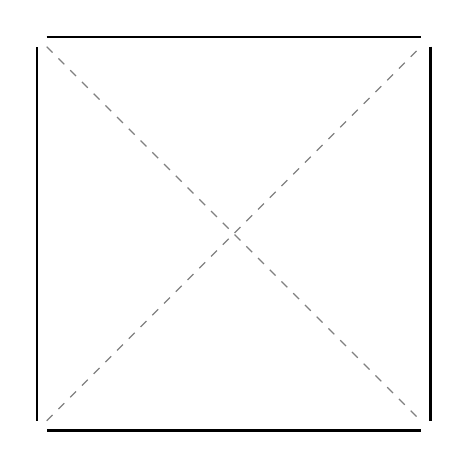
\begin{tikzpicture}
    \draw
		node (1) at (0, 0) {}
        node (2) at (0, \x) {}
        node (3) at (\x, \x) {}
        node (4) at (\x, 0) {}
    ;
    \draw
        [thick]
        (1) -- (2) -- (3) -- (4) -- (1)
    ;
    
    \draw
        [dashed, gray]
        (1) -- (3)
        (2) -- (4)
    ;
\end{tikzpicture}
\hspace{0.5cm}
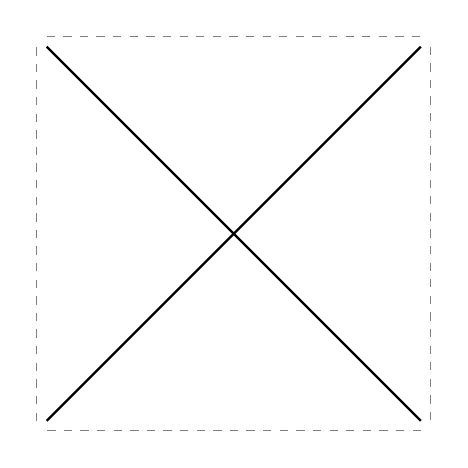
\begin{tikzpicture}
    \draw
        node (1) at (0, 0) {}
        node (2) at (0, \x) {}
        node (3) at (\x, \x) {}
        node (4) at (\x, 0) {}
    ;
    \draw
        [dashed, gray]
        (1) -- (2) -- (3) -- (4) -- (1)
    ;
    \draw
        [thick]
        (1) -- (3)
        (2) -- (4)
    ;
\end{tikzpicture}
\end{document}